\documentclass[12pt]{article}
\usepackage{fontspec}      % Allows loading system fonts
\setmainfont{Arial}        % Sets the default body text font to Arial
\usepackage{graphicx}      % Required for inserting images
\usepackage[margin=1in]{geometry}
\usepackage{underscore}    % this allows use of underscore without subscripting
\usepackage{float}         % use to fix figures

\begin{document}

\begin{center}
    {\Large \textbf{Predicting Battery Useful Life}\par}
    \vspace{2em}
    {\large CS342 Project Report\par}
    \vspace{1.5em}
    {Leo Lin 5592102\par}
\end{center}

\section{Task 1: Exploratory Data Analysis and Data Visualisation}

\subsection{Characteristics of the data}

\begin{figure}[H]
    \centering
    \makebox[\textwidth][c]{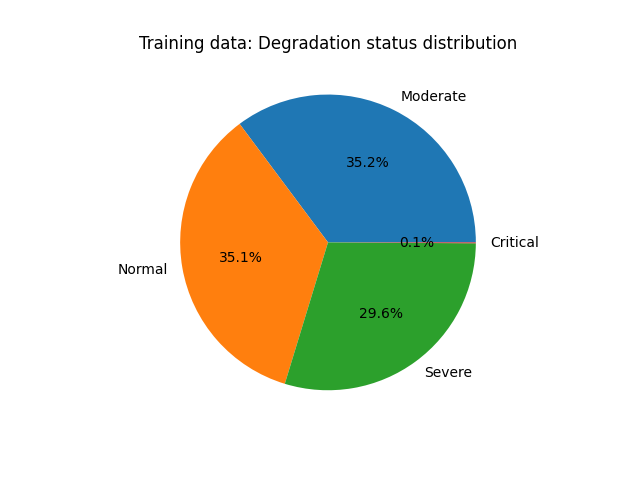
\includegraphics[width=0.65\textwidth]{deg_pie_char.png}}
    \caption{Percentage of each degradation status in the training data}
    \label{fig:pie}
\end{figure}

The figure above shows there is a massive class imbalance in the training data. Additionally, the data has no missing values for any features other than 'pack_temp_c'. Fig 2 later in the report shows that we can use 'ambient_temp_c' as a substitute for this.

\subsection{Correlation Analysis}

It is important to analyse the correlation between covariates in the data as a high correlation between covariates could cause multicollinearity which could affect the weighting of some covariates. This can be done using a correlation heat map.

\begin{figure}[H]
    \centering
    \makebox[\textwidth][c]{\includegraphics[width=1\textwidth]{corr_heatmap.png}}
    \caption{Covariates in battery observations and battery metadata}
    \label{fig:timetable}
\end{figure}

Figure 2 shows there is some high correlation between some of the covariates of the data. Most of the correlations can be inferred from the Kaggle data card about the columns.c 

\begin{itemize}
    \item Temperature such as 'pack_temp_c' and 'ambient_temp_c'.
    \item 'charge_current_a' and 'discharge_current_a' have high correlation with 'charge_c_rate' and 'discharge_c_rate' respectively;
    \item Energy statistics such as 'energy_discharged_kwh' are highly correlated with each other.
    \item 'battery_age_days' and 'cycle_index' are highly correlated with usage of the battery.
\end{itemize}

\subsection{Feature separability by degradation status}

Visualising covariates by 'degradation_status' can help find patterns or trends that could identify 'degradation status'. Covariates that were not shown in this plot were categorical covariates; covariates that were highly related to a covariate already in the plot; and irrelevant covariates.

\begin{figure}[H]
    \centering
    \makebox[\textwidth][c]{\includegraphics[width=1\textwidth]{covariate_analysis.png}}
    \caption{Feature separability by degradation status}
    \label{fig:timetable}
\end{figure}

Some covariates show different patterns depending on 'degradation status'

\begin{itemize}
    \item Usage seems like the most important factor for determining 'degradation_status'. 'equivalent_full_cycles' has a median of about 70 for 'Normal', 210 for 'Moderate' and 350 for 'Severe' and 'Critical'. This indicates an old battery is likely to be in a degraded state.
    \item 'ambient_temp_c' has an unusual median for 'Critical' status. This is most likely an anomaly since 'Critical' batteries having lower 'ambient_temp_c' makes little sense and could be caused by 'Critical' having a low class count.
\end{itemize}




'cumulative_high_temp_hours' has an increasing amount of high values for more degraded batteries. This feature might be useful.

\subsection{Degradation status by categorical features}

Analysing how degradation status changes across categorical features is important. To visualise this we can use a stacked bar chart.

\begin{figure}[H]
    \centering
    \makebox[\textwidth][c]{\includegraphics[width=1\textwidth]{categorical_analysis.png}}
    \caption{Percentage of each degradation status by categorical features}
    \label{fig:timetable}
\end{figure}

'eol_reached' and 'usage_strategy' both appear to be highly predictive features for 'degradation_status'. In this plot 0 is False and 1 is True, when a battery reaches end of life it most likely means heavy usage and relates to the pattern that covariates that track usage are highly predictive of the degradation status.

\section{Task 2: Unsupervised (Classic) Machine Learning for Battery Degradation Analysis}

\subsection{Feature selection and preprocessing}

Using patterns inferred from task 1 and testing combinations of parameters these parameters were found to be predictive of 'degradation_status':

\begin{itemize}
    \item 'eol_reached', when this feature is True the probability of the degradation status being critical or severe is significantly higher. Encode this feature as 1 when true and 0 when false.
    \item 'equivalent_full_cycles', this feature is the best feature for determining how used the battery was.
    \item 'usage_strategy' was seen to be predictive in Figure 3 of a worsening degradation status. This data was encoded as an ordinal variable with 'Conservative' as 1 and 'Aggressive' as 4.
\end{itemize}

Testing revealed that using more than these 3 features significantly reduced accuracy.

Using GMM means that the features need to be normalised otherwise large scale features can dominate other features. The training data is used to standardise the features of validation and test data as well as to prevent data leakage.

\subsection{Unsupervised Learning Model}

For this task a GMM (Gaussian Mixture Models) was chosen, since from testing k-means on the data it shows that the spherical assumption of k-means does not work well on the data. GMM is more flexible and allows for non-spherical-shaped clusters which fit the data much better.

The clusters will be set to the class that is most present in the cluster (majority voting), because of the class imbalance shown in Fig 1 however, this means 'Critical' class will not be predicted.

Testing values of n_components showed that over-clustering was the best approach.

\begin{center}
\begin{tabular}{||c c c c||} 
 \hline
 n_components & AIC & BIC & Validation Error \\ [0.5ex] 
 \hline\hline
 60 & -2289737.4 & -2283918.7 & 16.81\% \\
 \hline
 70 & -2289852.1 & -2283062.2 & 16.32\% \\
 \hline
 80 & -2289939.3 & -2282178.0 & 16.67\% \\
 \hline
 90 & -2289867.8 & -2281135.1 & 16.10\% \\
 \hline
 100 & -2289866.6 & -2280162.5 & 16.93\% \\
 \hline
\end{tabular}
\end{center}

In testing, the 'full' covariance type was the best since it provided the best flexibility which is needed for this data. The n_component used in the model was 90 since it minimised the validation error.

\begin{figure}[H]
    \centering
    \makebox[\textwidth][c]{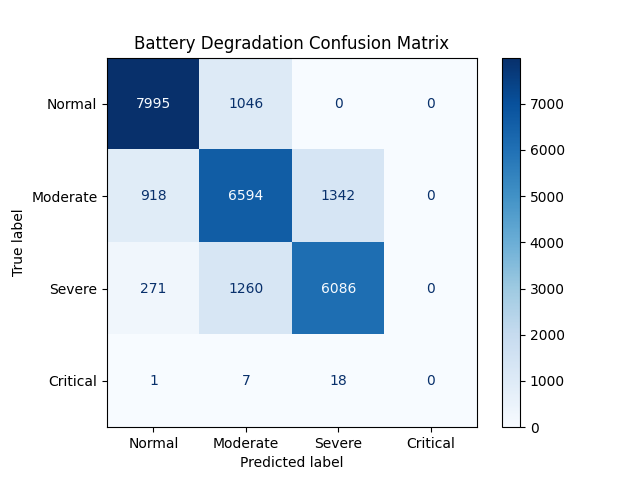
\includegraphics[width=0.7\textwidth]{confusion_matrix_1.png}}
    \caption{Confusion matrix for test set (Accuracy: 81.0\%)}
    \label{fig:timetable}
\end{figure}

\subsection{Analysis of results}

The accuracy of the model was 80.96\% in the test data set. It is very difficult for a clustering algorithm to detect the small 'Critical' class with majority voting but this cluster to class approach improved the rest of the class accuracies significantly. The model tends to 'underestimate' the degradation status and predicts 'Normal' for lots of 'Moderate' points and 'Moderate' for 'Severe' points. This indicates how there is little change between a single stage of change in the degradation status as it was the most common error for the model. Overall, the cluster groups do correspond to meaningful battery degradation behaviour.

\subsection{Usefulness of features}

The features considered for the model were 'equivalent_full_cycle', 'eol_reached', 'usage_strategy' and 'cumulative_high_temp_hours'. Task 1 showed these features could be useful. Compare usefulness by dropping covariates one at a time.

\begin{center}
\begin{tabular}{||c c c c||} 
 \hline
 Model & AIC & BIC & Validation Error \\ [0.5ex] 
 \hline\hline
 All 4 covariates included & -3001961.6 &-2988857.6 & 27.90\% \\ 
 \hline
 'equivalent_full_cycle' removed & -3201081.7 & -3192349.0 & 44.84\% \\ 
 \hline
 'cumulative_high_temp_hours' removed & -2289867.8 & -2281135.1 & 16.10\% \\ 
 \hline
 'eol_reached' removed & -1581716.7 & -1572983.9 & 29.73\% \\
 \hline
 'usage_strategy' removed & -1682727.5 & -1673994.8 & 22.02\% \\
 \hline
\end{tabular}
\end{center}

This shows that 'cumulative_high_temp_hours' was a noisy feature for this model and that 

'cumulative_high_temp_hours' was the least impactful feature. 'equivalent_full_cycle' was the most important feature by far as removing it made the error of the model extremely high. Both 'eol_reached' and 'usage_strategy' were not as useful as 'equivalent_full_cycle' but still improved the model with the inclusion.

\section{Task 3: Supervised (Classic) Machine Learning for Battery Degradation Analysis}

This task will be done with XGBoost classifier.

\subsection{Feature selection and engineering}

The features that were good in task 2 will be used in this model as well. Adding more features such as 'ambient_temp_c', 'cumulative_high_temp_hours' and 'depth_of_discharge_pct' as battery stress factors could be good. This model has regularization, so noisy features won't affect the model as much unlike GMM.

Similar data preprocessing techniques are used here as in task 1 so categorical features such as 'eol_reached' and 'usage_strategy' are encoded as ordinal variables.

The data card explains that the internal resistance of the pack increases as the battery degrades so 'resistance_growth' could be a good feature to add. This feature is calculated as 'internal_resistance_mOhm' / ('cycle_index' + 1).

XGBoost doesn't require standardised features unlike the previous model so we can keep all features as they are.

\subsection{Supervised Learning Model}

Unlike the unsupervised learning model in task 2, this model will be trained to learn the 'Critical' degradation status since supervised learning models are given target labels, which means they can more easily identify this narrow 0.1\% of the data.

Grid Search was used for hyperparameter tuning and finds the best combination of hyperparameters to maximise macro F1 score. In addition, the built-in 'early_stopping_rounds' hyperparameter stops the model when increasing 'n_estimators' doesn't improve the validation loss.

\begin{center}
\begin{tabular}{||c c c||} 
 \hline
 Hyperparameter & Search Space & Optimal Value \\ [0.5ex] 
 \hline\hline
 max\_depth & [3, 5, 7, 9] & 5 \\ 
 \hline
 min\_child\_weight & [1, 3, 6] & 5 \\ 
 \hline
 subsample & [0.6, 0.7, 0.8, 1.0] & 0.8 \\ 
 \hline
 colsample\_bytree & [0.6, 0.7, 0.8, 1.0] & 0.8 \\ 
 \hline
 reg\_alpha & [0.0, 0.1, 0.5, 1.0] & 0.5 \\ 
 \hline
 learning\_rate & [0.01, 0.03, 0.05, 0.1] & 0.05 \\ 
 \hline
 n\_estimators & [300, 500, 1000] & 1000 \\ 
 \hline
\end{tabular}
\end{center}

\subsection{Evaluation of the model}

Macro F1 score is the best evaluation metric to use since this is a classification problem. This is the confusion matrix for the model that maximised macro F1.

\begin{figure}[H]
    \centering
    \makebox[\textwidth][c]{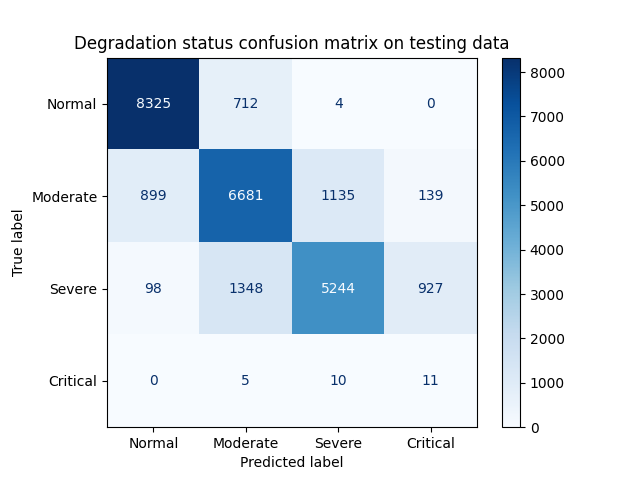
\includegraphics[width=0.7\textwidth]{confusion_matrix_2.png}}
    \caption{Confusion matrix for test set (Accuracy: 85.56\%)}
    \label{fig:timetable}
\end{figure}

The recall and precision of 'Critical' is low, when the model predicts 'Critical' it is most of the time a 'Severe' point. The model performs very well on the other 3 classes, especially 'Normal'.

\subsection{Feature importance}

\begin{center}
\begin{tabular}{||c c c c||} 
 \hline
 Feature & Gain & Weight & Cover \\ [0.5ex] 
 \hline\hline
 eol\_reached & 125.435112 & 1608.0 & 4413.442383 \\ 
 \hline
 equivalent\_full\_cycles & 99.647728 & 11297.0 & 3765.045654 \\ 
 \hline
 usage\_strategy & 47.151421 & 3219.0 & 3048.288574 \\ 
 \hline
 resistance\_growth & 44.798866 & 9023.0 & 2302.284180 \\ 
 \hline
 depth\_of\_discharge\_pct & 42.865730 & 4815.0 & 2514.131592 \\ 
 \hline
 ambient\_temp\_c & 39.376331 & 8320.0 & 2595.524902 \\ 
 \hline
 cumulative\_high\_temp\_hours & 32.494751 & 7254.0 & 3034.156006 \\ 
 \hline
\end{tabular}
\end{center} 

The table shows the features that were good in the unsupervised model are still good in this model. Each feature is shown to have either good gain or weight. Highly useful features such as 'equivalent_full_cycles' have both of these values high. 

\section{Task 4: Unsupervised Deep Learning for Battery Degradation Analysis}

This task will be completed using improved deep embedded clustering (IDEC). The model framework and training was created by generative AI.

\subsection{Preprocessing and model design}

The best features are 'equivalent_full_cycles', 'eol_reached' and 'usage_stategy' as seen in task 2 and 3, however standard IDEC uses MSE loss which performs poorly with discrete features, so for this model 'eol_reached' and 'usage_strategy' are omitted. Task 3 showed that 'resistance_growth', 'depth_of_discharge_pct', 'ambient_temp_c' and 'cumulative_high_temp_hours' are somewhat informative.

IDEC model requires features to be standardised before effective use. So, the features are standardised using sklearn.StandardScalar before being used in the model so that no features dominate.

Hyperparamer tuning:

\begin{itemize}
    \item Latent space was tested at 2, 3 and 4. Latent space at 4 maximised macro F1 score.
    \item Gamma is a weighting coefficient that balances clustering loss and reconstruction loss, by default it is set to 0.1. The default is good and creates the best balance in clusters from my testing.
    \item Noise_std is the standard deviation of the Gaussian noise added to input data, this value is set to 0.15 to force autoencoder to learn patterns in the data.
    \item n_clusters, since task 2 showed over-clustering helped, the approach was to start with high clusters and work down. n_clusters=6 was a good fit for the data.
\end{itemize}

The selected training procedure was the typical procedure for IDEC, which was pretraining the denoising autoencoder using reconstruction loss and then running K-means to initialise cluster centres on the latent space. The next stage of training is joint reconstruction and clustering optimisation to minimise the combined loss function. This procedure is recommended for tabular data and for quite low-dimension data which this problem fitted.

The clusters are then assigned to labels that are most common inside the cluster (majority voting).

\subsection{Analysis and interpretation of the learned representations}

\begin{figure}[H]
    \centering
    \makebox[\textwidth][c]{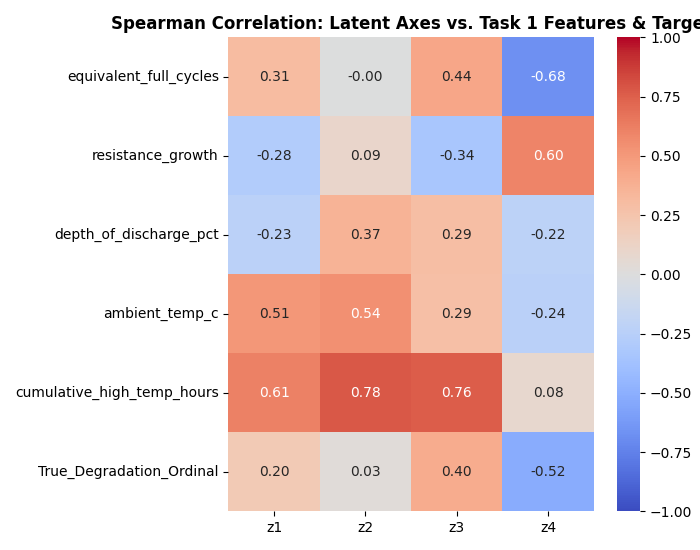
\includegraphics[width=1\textwidth]{latent_corr.png}}
    \caption{Features correlation with latent space dimensions}
    \label{fig:timetable}
\end{figure}

This figure shows the correlation of the features with the dimensions in the latent space.

\begin{itemize}
    \item z1 represents 'cumulative_high_temp_hours' in the latent space. This factor has a low correlation with degradation status.
    \item z2 captures the amount of cycles the battery has been used for, as expected for a usage factor, it has high correlation with degradation status.
    \item z3 represents the heat stress of the battery. This factor has no correlation with degradation status.
    \item z4 represents the usage of the battery as it had high correlation with all usage features, as other tasks have shown, usage is the most important factor and this made z4 the best latent factor for clustering.
\end{itemize}

\subsection{Usefulness of features}

'equivalent_full_cycles', 'cumulative_high_temp_hours' and 'resistance_growth' are the most useful features and all had high correlation with the latent dimensions. Just like the tasks before, this shows that the usage of the battery is the most important factor for evaluating the degradation status. 'cumulative_high_temp_hours' performs surprisingly well in the latent space, unlike in task 2 and task 3 this features was very useful.

'ambient_temp_c' was slightly useful and captured the heat stress of the battery, it was used in most latent factors. 'depth_of_discharge_pct' was not useful for this model and had low correlation with all latent factors. These two features are consistently lower impact than other features in task 2 and task 3.

\section{Task 5: Supervised Deep Learning for Battery Degradation Analysis}

A good supervised deep learning model for predicting degradation status is TabPFN.

\subsection{Supervised Deep Learning Model}

\subsection{Preprocessing, architecture and training strategy}

\subsection{Evaluation of classification performance}

\subsection{Comparison with task 3 and feature relevance}

\end{document} 